\documentclass[12pt,a4paper]{report}

\input{var.tex}

%======================= PACKAGES =======================
\usepackage{fontspec}              % requires XeLaTeX or LuaLaTeX
\usepackage[top=1in,bottom=1in,left=1.25in,right=1in]{geometry}
\usepackage{tocloft}
\usepackage{setspace}
\usepackage{titlesec}
\usepackage{graphicx}
\usepackage{caption}
\usepackage{float}
\usepackage{fancyhdr}
\usepackage{enumitem}
\usepackage{chngcntr}
\usepackage[table]{xcolor}
\usepackage[hidelinks]{hyperref}
\usepackage{amsmath}
\usepackage{algorithm}
\usepackage{algpseudocode}

\graphicspath{{../images}}

%======================= FONT =======================
\setmainfont{Times New Roman}

%======================= FIGURE / TABLE NUMBERING =======================
\counterwithout{figure}{chapter}
\counterwithout{table}{chapter}
\numberwithin{figure}{chapter}
\numberwithin{table}{chapter}

%======================= CAPTION STYLE =======================
\DeclareCaptionFont{twelvept}{\fontsize{12}{14}\selectfont}

% Figure and table captions: centered, bold, 12pt, below
\captionsetup[figure]{
  font={bf,twelvept},
  labelfont=bf,
  textfont=bf,
  justification=centering,
  singlelinecheck=true,
  position=bottom,
  skip=8pt
}

\captionsetup[table]{
  font={bf,twelvept},
  labelfont=bf,
  textfont=bf,
  justification=centering,
  singlelinecheck=true,
  position=bottom,
  skip=8pt
}

%======================= HEADING STYLES =======================
\titleformat{\chapter}[block]
  {\normalfont\bfseries\setstretch{1}\fontsize{16}{19}\selectfont\centering}
  {}
  {0.5em}
  {}
\titlespacing*{\chapter}{0pt}{-16pt}{0pt}

\titleformat{\section}
  {\normalfont\bfseries\fontsize{14}{17}\selectfont}
  {\thesection}{10pt}{}
\titlespacing*{\section}{0pt}{18pt}{10pt}

\titleformat{\subsection}
  {\normalfont\bfseries\fontsize{12}{15}\selectfont}
  {\thesubsection}{10pt}{}
\titlespacing*{\subsection}{0pt}{14pt}{8pt}

%======================= TOC =======================
\renewcommand{\cftchapfont}{\bfseries}
\renewcommand{\cftchappagefont}{\bfseries}
\renewcommand{\cftchapdotsep}{\cftdotsep}
\renewcommand{\cftchapaftersnum}{.}
\renewcommand{\cftsecaftersnum}{}
\renewcommand{\cftsubsecaftersnum}{}

\renewcommand{\cftsecfont}{\normalfont}
\renewcommand{\cftsecpagefont}{\normalfont}
\renewcommand{\cftsubsecfont}{\normalfont}
\renewcommand{\cftsubsecpagefont}{\normalfont}

\setlength{\cftbeforetoctitleskip}{-16pt}
\renewcommand{\contentsname}{TABLE OF CONTENTS}
\renewcommand{\cfttoctitlefont}
  {\hfill\bfseries\setstretch{1}\fontsize{16}{19}\selectfont}
\renewcommand{\cftaftertoctitle}{\hfill}

%======================= LIST OF FIGURES / TABLES =======================
% Titles: centered, same style as the TOC title
\renewcommand{\cftloftitlefont}
  {\hfill\bfseries\setstretch{1}\fontsize{16}{19}\selectfont}
\renewcommand{\cftafterloftitle}{\hfill}

\renewcommand{\cftlottitlefont}
  {\hfill\bfseries\setstretch{1}\fontsize{16}{19}\selectfont}
\renewcommand{\cftafterlottitle}{\hfill}

\renewcommand{\cftfigpresnum}{Figure }
\renewcommand{\cftfigaftersnum}{}
\setlength{\cftfignumwidth}{6.2em}
\renewcommand{\cftfigfont}{\normalfont}
\renewcommand{\cftfigpagefont}{\normalfont}

\renewcommand{\cfttabpresnum}{Table }
\renewcommand{\cfttabaftersnum}{}
\setlength{\cfttabnumwidth}{6.2em}
\renewcommand{\cfttabfont}{\normalfont}
\renewcommand{\cfttabpagefont}{\normalfont}
\setlength{\cftbeforeloftitleskip}{-16pt}
\setlength{\cftbeforelottitleskip}{-16pt}

%======================= PAGE NUMBERING =======================
\pagestyle{fancy}
\fancyhf{}
\fancyfoot[C]{\thepage}
\renewcommand{\headrulewidth}{0pt}

\fancypagestyle{plain}{%
  \fancyhf{}
  \fancyfoot[C]{\thepage}
  \renewcommand{\headrulewidth}{0pt}
}

%======================= MISC =======================
\setlength{\parindent}{0pt}
\setlength{\parskip}{1\baselineskip}

%======================= FLOAT SPACING =======================
\setlength{\intextsep}{6pt plus 2pt minus 2pt}      % above/below [H] floats
\setlength{\floatsep}{8pt plus 2pt minus 2pt}
\setlength{\textfloatsep}{8pt plus 2pt minus 2pt}

% No paragraph or list spacing inside figure/table/algorithm environments
\makeatletter
\g@addto@macro\@floatboxreset{%
  \setlength{\parskip}{0pt}%
  \setlength{\topsep}{0pt}%
  \setlength{\partopsep}{0pt}%
}
\makeatother


\begin{document}

%======================= COVER PAGE =======================
\begin{titlepage}
\centering
\thispagestyle{empty}


\includegraphics[height=4.6cm]{Tribhuvan-University-Logo.png}

{\fontsize{16}{19}\selectfont\bfseries
Tribhuvan University\par}

{\fontsize{14}{17}\selectfont\bfseries
Faculty of Humanities and Social Sciences\par}

\vspace{0.8cm}

{\fontsize{14}{17}\selectfont\bfseries
Ches: Online Chess Game Using .NET, Raylib and PostgreSQL\\
with Difficulty based AI Player\par}

\vspace{0.8cm}
{\fontsize{13}{16}\selectfont\bfseries
A PROJECT REPORT\par}
\vspace{0.8cm}

{\fontsize{12}{15}\selectfont
\bfseries Submitted to\par
\vspace{2pt}
\bfseries Department of Computer Application\par
\bfseries \COLLEGE \par}

\vspace{0.8cm}

{\fontsize{12}{15}\selectfont\itshape
\bfseries In partial fulfillment of the requirements for the Bachelors in Computer Application\par}
\vspace{0.8cm}

{\fontsize{12}{15}\selectfont
Submitted By\par

\FIRSTNAME \space  \LASTNAME \space [TU Reg No: \TUID]\par
October, 2026\par}

\vfill

\end{titlepage}

%======================= FRONT MATTER =======================
\pagenumbering{roman}
\setcounter{page}{1}
\onehalfspacing


\tableofcontents
\newpage
\listoffigures
\newpage
\listoftables

\pagenumbering{arabic}
\setcounter{page}{1}


\chapter{INTRODUCTION}
\label{ch:introduction}

Chess is one of the oldest and most widely played strategy games in the world. With the growth of the internet, chess has moved from the physical board to online platforms where players can find opponents from anywhere at any time. A good online chess platform must do more than display a board. It must enforce the rules of the game correctly, keep both players synchronized in real time, store game records, and match players with opponents of similar strength so that games remain interesting and fair.

The Multiplayer Chess Game is a desktop application developed using C\# on the .NET platform. The graphical interface, including the board, pieces, and menus, is built using Raylib, a simple and easy-to-use library for game programming. The game is presented in 2.5D. PostgreSQL is used as the database to store player accounts, games, moves, and ratings. The game follows a client-server architecture in which a central server validates moves and controls each match, while the game clients display the board and send player actions to the server.

In addition to online multiplayer, the system includes a Player versus Environment (PvE) mode in which the player competes against a computer opponent. The computer opponent is a neural network trained on a large collection of games played by strong human players. Given a board position, the network predicts the moves a strong player would be likely to choose, and the game selects among them according to the chosen difficulty level. This allows players to practice at any time, even when no human opponent is available.

To support competitive play, the system uses the Elo rating system. Every player has a numerical rating that changes after each completed online game depending on the result and the strength of the opponent. The matchmaking module uses these ratings to place players in a queue and pair them with opponents whose ratings are close to their own. The system also provides an administrative module for managing players and viewing game records. The main purpose of the project is to demonstrate how game development, networking, database management, a rating algorithm, and machine learning can be combined to build a complete chess game.


\chapter{PROBLEM STATEMENT}
\label{sec:problem}

\begin{itemize}[leftmargin=1.5em]
    \item Playing chess against another person normally requires both players to be in the same place or to use a large commercial online platform. Players who want to practice with others may be paired with opponents who are much stronger or much weaker than themselves, which makes games frustrating or unchallenging. Without a rating system, there is also no reliable way for players to measure their progress or compare their skill with others.
\end{itemize}


\chapter{OBJECTIVES}
\label{sec:objectives}

\begin{itemize}[leftmargin=1.5em]
    \item To develop a multiplayer chess game using .NET and Raylib in which players can compete online against opponents of similar skill selected by an Elo-based matchmaking system, with all player, game, and rating data stored in a PostgreSQL database.
\end{itemize}


\chapter{METHODOLOGY}
\label{ch:methodology}
\section{Development Model}

The project will be following Waterfall with incremental development methodology for its simplicity, fast development time. It has advantage over agile where we do not need to wait for feedback from users. We can simply iterate over using waterfall model as a basis quick. This gives us advantage of waterfall while providing us with flexibility that we need.

\begin{figure}[H]
  \centering
  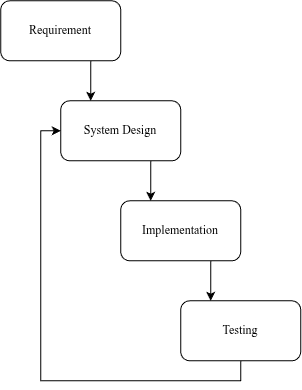
\includegraphics[width=11cm,keepaspectratio]{waterfall.png}
  \caption{Waterfall Model for Multiplayer Chess Game}
  \label{fig:waterfall}
\end{figure}


\section{Requirement Identification}
\label{sec:reqid}

\subsection{Study of Existing System}
\label{sec:existing}

Chess has long been played over the board under the rules maintained by the International Chess Federation (FIDE) \cite{fide}. The game has a long history and developed into its modern form in Europe in the fifteenth century. In traditional over-the-board chess, players must meet in the same place, find opponents of suitable strength by themselves, and record games by hand. Official ratings are issued by FIDE and national federations, and they are updated only after rated tournaments \cite{fide}. Because of this, the feedback a player receives is slow and depends on tournament access.

Online platforms removed many of these limitations. Two of the most widely used are Chess.com and Lichess.

\textbf{Chess.com} is a commercial platform that offers live and daily games, puzzles, lessons, and computer opponents with different playing personalities. It uses a Glicko-based rating system \cite{chesscomrating}, and a basic account is free, but many analysis and learning features require a paid subscription.

\textbf{Lichess} is a free, non-profit, and open-source platform with no advertisements \cite{lichess}\cite{lila}. It pairs players through a rating-based matchmaking lobby and rates them using the Glicko-2 system \cite{glickman2001dynamic}. It also offers play against the Stockfish engine at several levels \cite{stockfish}, and it publishes all rated games in an open database.

Both platforms are large web-based services built for very large numbers of players. They are designed for web browsers and mobile applications, and their server software is complex. Chess.com's server code is not public. Lichess's code is public, but it is a large codebase that is hard to study in a short academic project. Their computer opponents are mostly based on search engines such as Stockfish, which calculate many moves ahead, rather than on models that imitate human move choices \cite{maia2020}.

\begin{table}[H]
\centering
\small
\renewcommand{\arraystretch}{1.25}
\begin{tabular}{|p{2.9cm}|p{3.4cm}|p{3.4cm}|p{3.4cm}|}
\hline
\textbf{Feature} & \textbf{Traditional (OTB)} & \textbf{Chess.com / Lichess} & \textbf{Proposed System} \\ \hline
Platform & Physical board & Web and mobile & Desktop \\ \hline
Finding opponents & Arranged manually or via tournaments & Automatic matchmaking & Elo-based matchmaking queue \\ \hline
Rating system & Elo (FIDE), updated per tournament & Glicko / Glicko-2, updated per game & Elo, updated per game \\ \hline
Computer opponent & None & Search-based engines, bots & Neural network with selectable difficulty \\ \hline
\end{tabular}
\caption{Comparison of existing chess systems with the proposed system}
\label{tab:comparison}
\end{table}

The study shows that existing platforms already offer reliable play, but they are large and complex, and their setup cannot easily be reproduced or studied. The proposed system implements their core features at a smaller scale: rule enforcement, rated matchmaking, stored game history, and a computer opponent. It combines these in a single desktop application with a 2.5D interface and an AI that imitates human play.

\subsection{Literature Review}
\label{sec:lit}

Arpad Elo introduced a statistical method for rating chess players in which each player has a numerical rating and the expected result of a game is calculated from the rating difference between the two players. After a game, ratings are adjusted according to the difference between the actual result and the expected result. This method became the basis of the rating systems used in chess and in many other competitive games \cite{elo1978rating}.

Glickman extended the idea of rating players by adding a measure of uncertainty, called the rating deviation, to each rating. Players who have played few games or have not played for a long time have a less reliable rating, and their ratings change more quickly. This improvement is used in the Glicko family of rating systems.

Online chess platforms such as Lichess allow players from around the world to play against each other with automatic matchmaking and rating updates. Lichess is a free and open-source platform and demonstrates how a rating system, a game server, and a database can be combined to support large numbers of online players \cite{lichess}.

The Lichess Open Database provides millions of recorded games, together with player ratings and results, that are released for free use \cite{lichessdb}. Such data makes it possible to train machine learning models that imitate human play. The Maia Chess project showed that neural networks trained on human games from a given rating range can predict human moves with good accuracy and can play in a more human-like way than traditional engines \cite{maia2020}. This project follows a similar approach on a smaller scale. The model is trained using the PyTorch library \cite{pytorch}, games are read using the python-chess library \cite{pythonchess}, and the trained model is exported in the ONNX format so that it can be executed inside a .NET application using ONNX Runtime \cite{onnxruntime}.

For the technical implementation, Raylib is a simple library for video game programming that provides functions for windowing, drawing, input, and audio, and can be used from C\# through available bindings \cite{raylib}. PostgreSQL is an open-source relational database system known for its reliability and standards compliance \cite{postgresql}, and Npgsql is the data provider that allows .NET applications to communicate with PostgreSQL. The rules that the game must implement are defined in the Laws of Chess published by the International Chess Federation \cite{fide}.

\subsubsection{Elo Rating and Matchmaking}
\label{sec:elo}

The system uses the Elo rating system to measure the skill of each player. Every new player starts with a default rating, and the rating changes after every completed game against another player. For a game between player A with rating $R_A$ and player B with rating $R_B$, the expected score of player A is calculated as follows \cite{elo1978rating}:

\begin{equation}
E_A = \frac{1}{1 + 10^{(R_B - R_A)/400}}
\end{equation}

After the game, the new rating of player A is calculated as:

\begin{equation}
R_A' = R_A + K\,(S_A - E_A)
\end{equation}

where $S_A$ is the actual score of player A (1 for a win, 0.5 for a draw, and 0 for a loss) and $K$ is a constant that controls how much a single game can change the rating. The rating of player B is updated in the same way. A player who defeats a stronger opponent gains more rating points than a player who defeats a weaker one. Games against the AI do not change the player's rating.

For matchmaking, a player who joins the queue is stored with the current rating and the time of joining. The server searches the queue for another player whose rating lies within an allowed range of the player's own rating. If no suitable opponent is found, the allowed range is gradually widened as the waiting time increases, so that players are not left waiting for too long. When a match is found, both players are removed from the queue, the colors are assigned, and a new game session is created.

\subsubsection{AI Opponent}
\label{sec:ai}

The computer opponent is implemented as a neural network that predicts the next move from a given board position. The development of the AI consists of the following stages.

\begin{itemize}[leftmargin=1.5em]
\item\textbf{Data Collection and Preprocessing}

Games are obtained from the Lichess Open Database in PGN format \cite{lichessdb}. Using the python-chess library \cite{pythonchess}, the games are filtered so that only standard games between players with high ratings (for example, above 1800) are kept. Each game is replayed move by move. Every position before a move is stored as an input, and the move chosen by the player is stored as the label. Each position is encoded as a set of some binary layers representing the pieces of each type and color, together with layers for castling rights and the en passant square, promotion, demotion. The board is oriented from the point of view of the player to move. Each move is encoded as a class index based on its start and end squares.

\item\textbf{Model Training}

A convolutional neural network is trained using PyTorch \cite{pytorch} to predict the played move from the encoded position. The data is divided into training and validation sets, and the model is evaluated using the accuracy of its move predictions on positions it has not seen before. Training is performed on a cloud GPU, and the trained model is exported to the ONNX format.

\item\textbf{Integration into the Game}

The game client loads the ONNX model using ONNX Runtime \cite{onnxruntime}. When it is the AI's turn, the rules engine provides the current position, which is encoded in exactly the same way as in training. The model outputs a score for each possible move. Scores of illegal moves are removed using the legal moves generated by the rules engine, so the AI can never make an illegal move.

\item\textbf{Difficulty Levels}

Difficulty is controlled without training separate models. The model's scores for the legal moves are converted into probabilities using a temperature value $T$:

\begin{equation}
P(m_i) = \frac{e^{z_i / T}}{\sum_j e^{z_j / T}}
\end{equation}

where $z_i$ is the model's score for legal move $m_i$. A low temperature makes the AI almost always select its best move, while a high temperature makes it select weaker moves more often. In addition, each difficulty level has a small probability of playing a random legal move to imitate human blunders. The combination of temperature and blunder probability defines the difficulty levels (for example, Easy, Medium, Hard, and Expert).
\end{itemize}

\subsection{Requirement Analysis}
\label{sec:reqanalysis}

Before designing the system, the functional and non-functional requirements were identified through a review of similar systems and an analysis of user needs.

\subsubsection{Functional Requirements}

\begin{enumerate}[label=\Roman*.]
    \item \textbf{User Registration and Login:} The system shall allow players to register and securely log in to the system.

    \item \textbf{Matchmaking:} The system shall allow a logged-in player to join a matchmaking queue and shall pair the player with an opponent of similar Elo rating.

    \item \textbf{Chess Gameplay:} The system shall allow two players to play a complete game of chess on a graphical board, with all moves validated according to the rules of chess.

    \item \textbf{Game Actions and Results:} The system shall support resigning, offering a draw, and detecting checkmate, stalemate, and other draw conditions to determine the result of a game.

    \item \textbf{Rating Update:} The system shall calculate and update the Elo rating of both players after each completed game between two human players.

    \item \textbf{Game and Rating History:} The system shall store completed games and the rating history of each player.

    \item \textbf{Admin Management:} The administrator shall be able to manage players and review game records.

    \item \textbf{Play Against AI:} The system shall allow a logged-in player to start a game against the computer opponent.

    \item \textbf{AI Difficulty Selection:} The system shall allow the player to select the difficulty level of the AI before the game begins.
\end{enumerate}

\textbf{Use Case Diagram}

\begin{figure}[H]
  \centering
  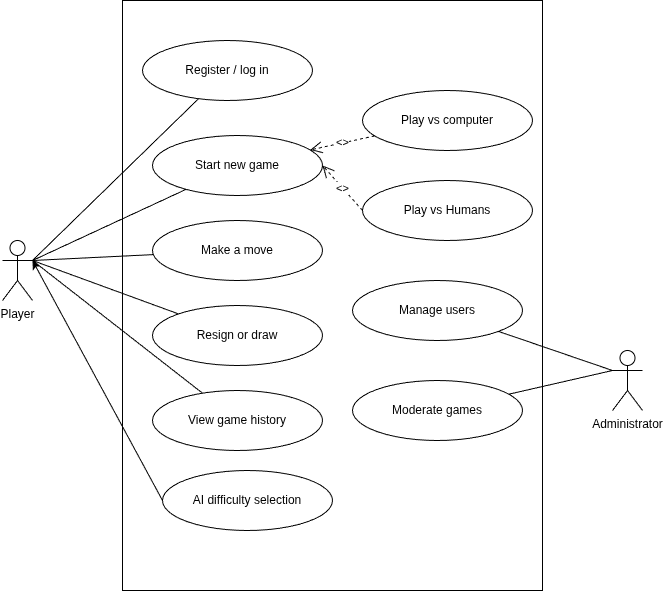
\includegraphics[height=10cm,keepaspectratio]{chess-use-case-diagram.png}
  \caption{Use Case Diagram of Multiplayer Chess Game}
  \label{fig:usecase}
\end{figure}

\subsubsection{Non-Functional Requirements}

\begin{enumerate}[label=\Roman*.]
    \item \textbf{Performance:} The system shall transmit and display moves with minimal delay so that gameplay feels responsive. The AI shall choose its move within a few seconds on a standard personal computer.

    \item \textbf{Usability:} The system shall provide a simple graphical interface for players to navigate.

    \item \textbf{Security:} The system shall store passwords in hashed form, validate all moves on the server, and restrict administrative functions to authorized users.

    \item \textbf{Integrity:} The system shall keep the game state consistent between both players and shall not lose completed game records.
\end{enumerate}

\section{Feasibility Study}
\label{sec:feasibility}

A feasibility study was carried out to determine whether the proposed Multiplayer Chess Game is practical, achievable, and suitable for implementation within the available resources. The feasibility of the system was examined from the following perspectives:

\subsection{Technical Feasibility:} The proposed system is technically feasible because it can be developed using the .NET platform and the C\# language, together with the open-source Raylib library for graphics and PostgreSQL for data storage. Network communication between the client and server can be implemented using standard socket support available in .NET. The system does not require expensive hardware, and a standard personal computer is sufficient for development and testing. The AI component is also technically feasible. Chess data is freely available from the Lichess Open Database, model training can be done in Python using free cloud GPU services such as Google Colab, and the trained model can be run in .NET through the ONNX Runtime package without requiring special hardware.

\subsection{Economic Feasibility:} The system is economically feasible because it can be developed using free and open-source software and tools. .NET, Raylib, PostgreSQL, and the required development tools are available without licensing costs, which keeps the overall development cost low and suitable for an academic project.

\subsection{Operational Feasibility:} The system is operationally feasible because the game is simple to use and follows familiar chess conventions. Players can register, log in, join the queue or start a game against the AI, and play with minimal instruction, and the administrator can manage players and game records through simple functions.

\section{High Level Design of System}
\label{sec:HighLevelDesignofSystem}

\subsection{Working Mechanism of The Proposed System}

\begin{figure}[H]
  \centering
  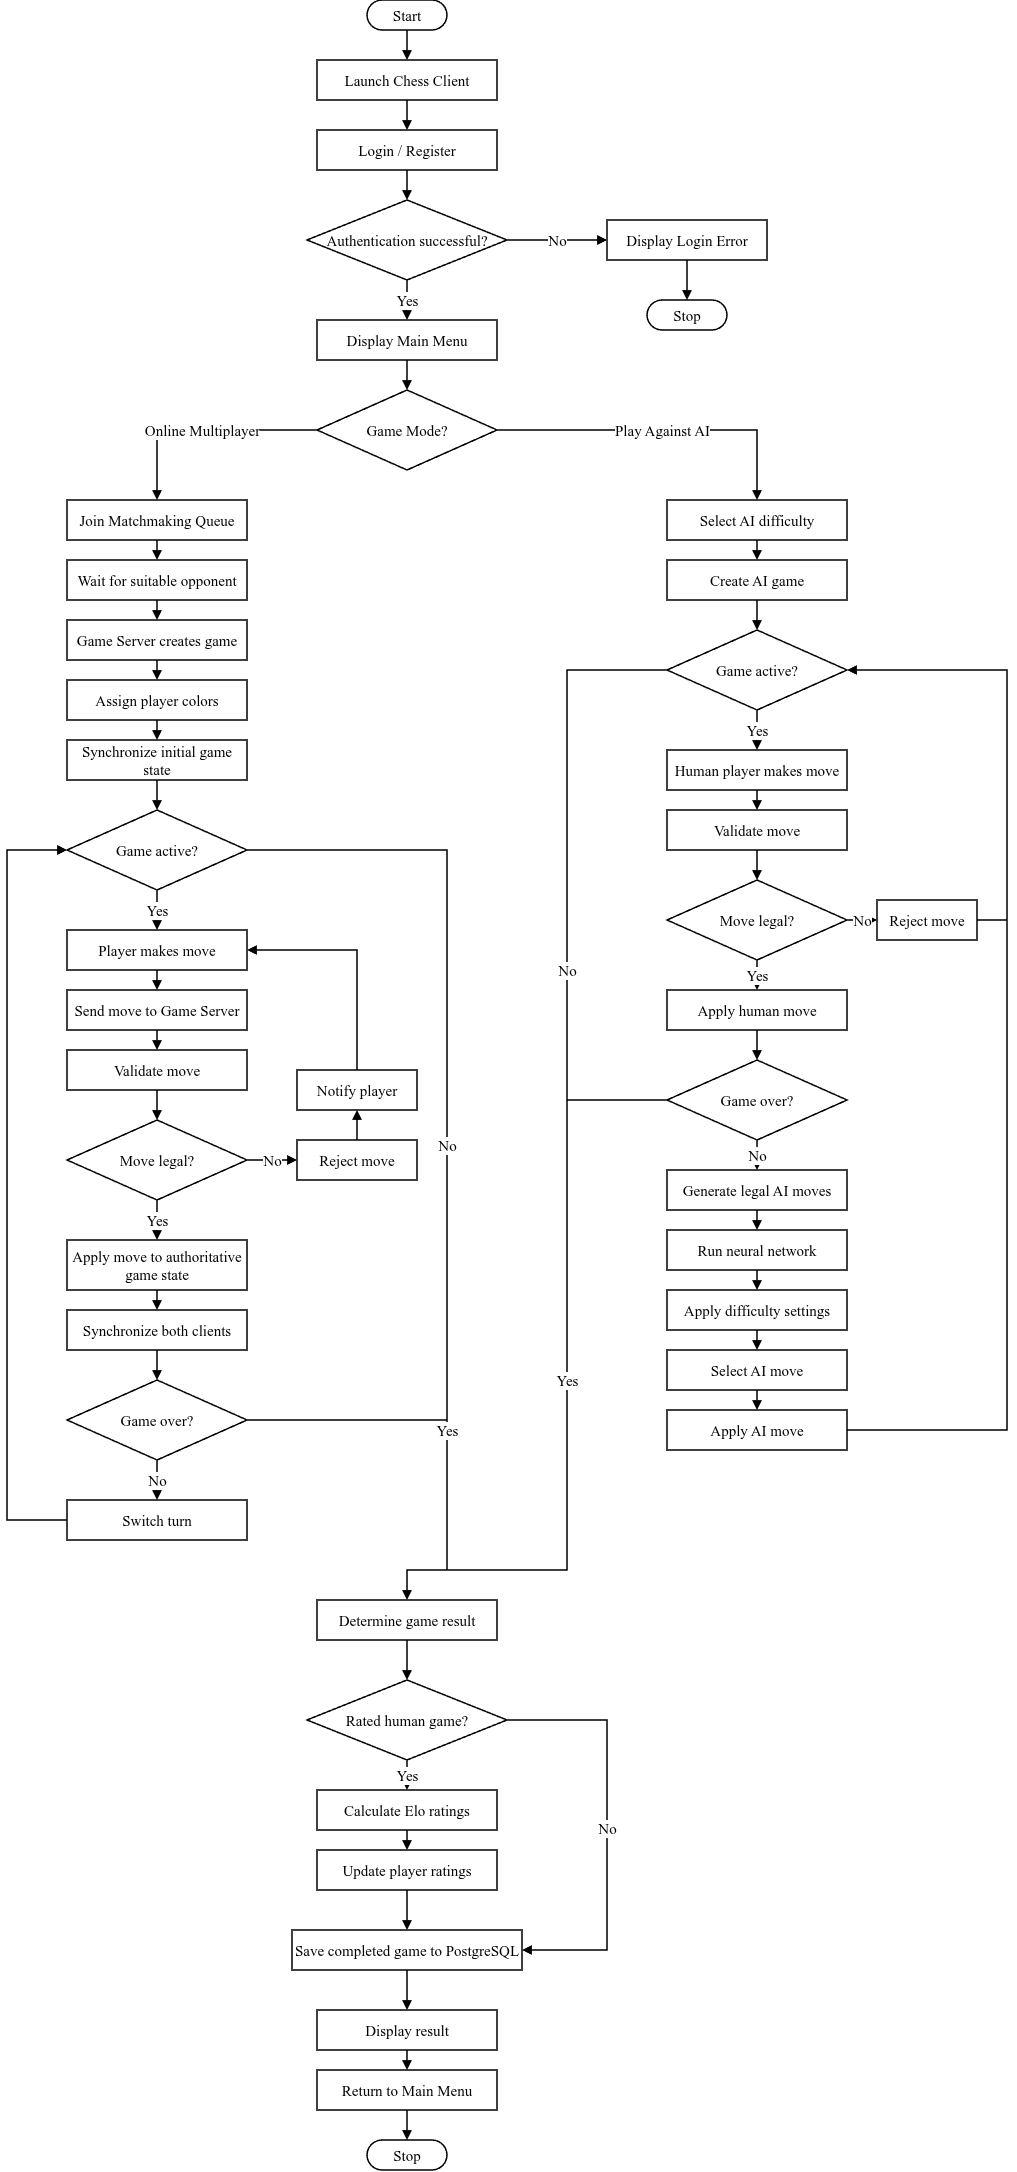
\includegraphics[width=15cm,height=19cm]{flowchart.png}
  \caption{Flow chart of Ches}
  \label{fig:flowchart}
\end{figure}


Figure~\ref{fig:flowchart} shows the overall workflow of the chess application, from launching the client to saving a completed game.

\textbf{Authentication}\\
The process begins when the user launches the chess client and logs in or registers. The system checks the credentials. If authentication fails, a login error is displayed and the process stops. If it succeeds, the main menu is displayed.

\textbf{Game mode selection}\\
From the main menu, the user chooses between two modes: Online Multiplayer and Play Against AI.

\textbf{Online multiplayer}\\
The player joins the matchmaking queue and waits for a suitable opponent. Once one is found, the game server creates the game, assigns colors to the players, and synchronizes the initial game state.

\textbf{Play against AI}\\
The player selects an AI difficulty, and the system creates an AI game. While the game is active, the human player makes a move, which is validated. An illegal move is rejected and the player tries again. A legal move is applied, and the system checks whether the game is over. If not, the AI takes its turn.

\textbf{Game completion}\\
When a game ends, in either mode, the system determines the result (win, loss, or draw). It then checks whether the game was a rated human game. If so, the Elo ratings are calculated and the player ratings are updated. AI games and unrated games skip this step. In all cases the completed game is saved to the PostgreSQL database, the result is displayed, and the user returns to the main menu before the process stops.


\subsection{Description of Algorithm}

\begin{algorithm}[H]
\caption{Elo Rating Update After a Completed Game}
\label{alg:elo}
\begin{algorithmic}[1]
\Require Ratings $R_A$ and $R_B$ of players $A$ and $B$; number of completed rated games
         $n_A$ and $n_B$ played by each player before this game; result $S_A \in \{1, 0.5, 0\}$
         (win, draw, loss for $A$)
\Ensure New ratings $R_A'$ and $R_B'$

\Function{KFactor}{$n$}
    \If{$n < 20$}
        \State \Return $25$ \Comment{new player: rating adjusts quickly}
    \ElsIf{$n < 70$}
        \State \Return $15$ \Comment{developing player}
    \Else
        \State \Return $7$ \Comment{established player: rating is stable}
    \EndIf
\EndFunction

\If{the game was played against the AI \textbf{or} the game was not completed}
    \State \Return $R_A,\ R_B$ \Comment{rating unchanged}
\EndIf
\State $S_B \gets 1 - S_A$
\State $E_A \gets \dfrac{1}{1 + 10^{(R_B - R_A)/100}}$ \Comment{expected score of $A$}
\State $E_B \gets 1 - E_A$ \Comment{expected score of $B$}
\State $K_A \gets \Call{KFactor}{n_A}$, \quad $K_B \gets \Call{KFactor}{n_B}$
\State $R_A' \gets R_A + \text{round}\big(K_A\,(S_A - E_A)\big)$
\State $R_B' \gets R_B + \text{round}\big(K_B\,(S_B - E_B)\big)$
\State $n_A \gets n_A + 1$, \quad $n_B \gets n_B + 1$
\State store $R_A'$, $R_B'$ and the updated game counts in the player records,
       and add a rating-history entry for each player
\State \Return $R_A',\ R_B'$
\end{algorithmic}
\end{algorithm}

In the above algorithm, we use a variable $K$-factor where
$K_f \in \{20,15,7\}$. When the player is new, the $K$-factor is
higher so that their Elo change is larger than normal. After 20 games,
it decreases to 15, and then to 7 after more than 70 games. This gives
new players time to reach their natural Elo rating more quickly.

The algorithm also uses lesser dividing value in the denominator of the original formula: $E_A = \dfrac{1}{1 + 10^{(R_B - R_A)/100}}$ instead of $E_A = \dfrac{1}{1 + 10^{(R_B - R_A)/400}}$ as lower value in dividor in denominator results in higher percent of punishment if lost by lower elo ranking player. and vice versa.


\subsection{Entity Relationship Diagram}

\begin{figure}[H]
  \centering
  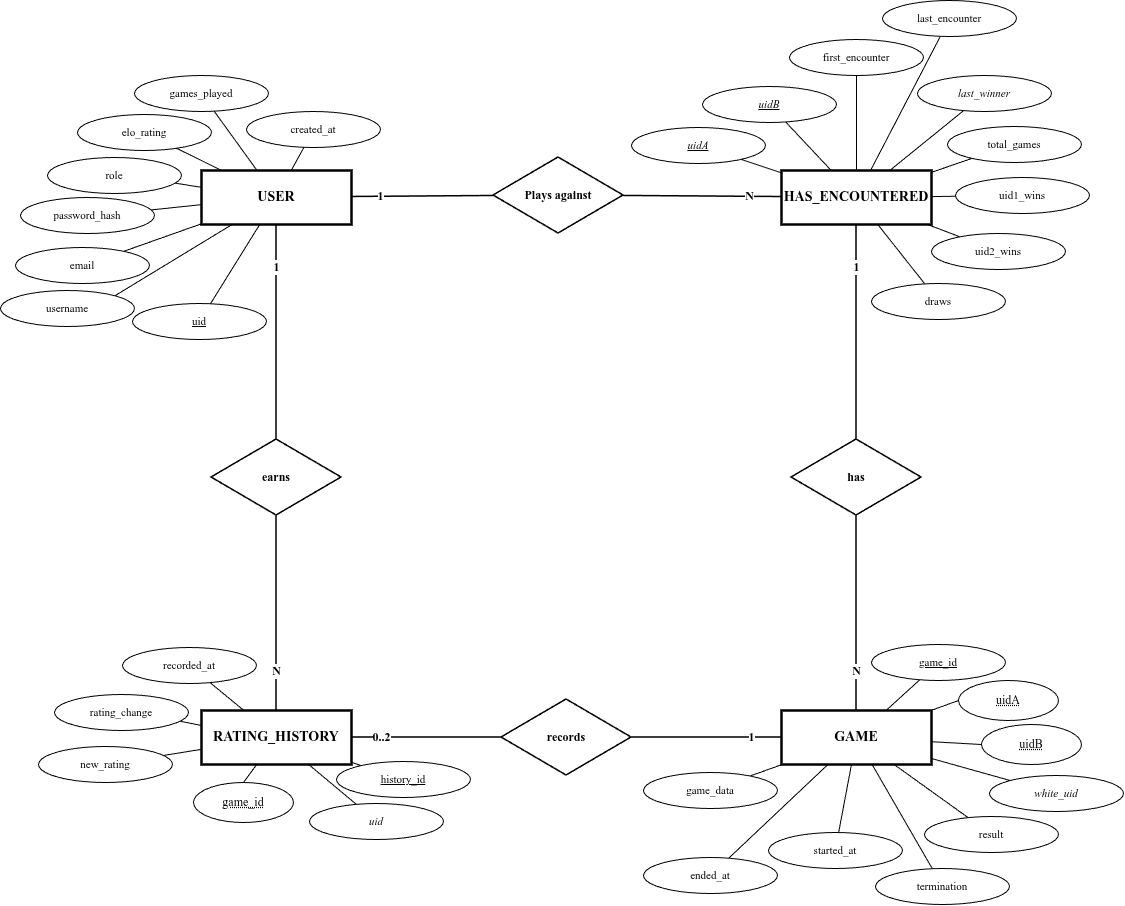
\includegraphics[height=15cm,width=15cm]{server-erd.png}
  \caption{Entity Relationship Diagram of Server}
  \label{fig:servererd}
\end{figure}

According to above figure, folowing entities are explained in points with their relationships with other entities.

\textbf{Users}\\
The User entity contains username, email, hashed password, elo etc. It contains all the data necessary to uniquely identify a user. Users plays agains other users. the players they have played against are stored on has\_encountered table. User is also related with rating history where each user's rating history is stored in the table.

\textbf{Has\_Encountered}\\
The entity contains keys of two user ids. They are composit primary key which has details like last winner, total games played, total draws, user\_1 wins, user\_2 wins and so on. This is usefull for maintaning statistical data of each user's opponent without having to recalculate them again. Has Encountered is related to game entity.

\textbf{Game}\\
This entity has gets the uidA and uidB from has\_Encountered then stores all the game movement data, start date, end date, termination, result, white\_uid and so on for game statistical history.

\textbf{Rating\_History}\\
Rating history tracks the changes of user rating with each games and its date.


\begin{figure}[H]
  \centering
  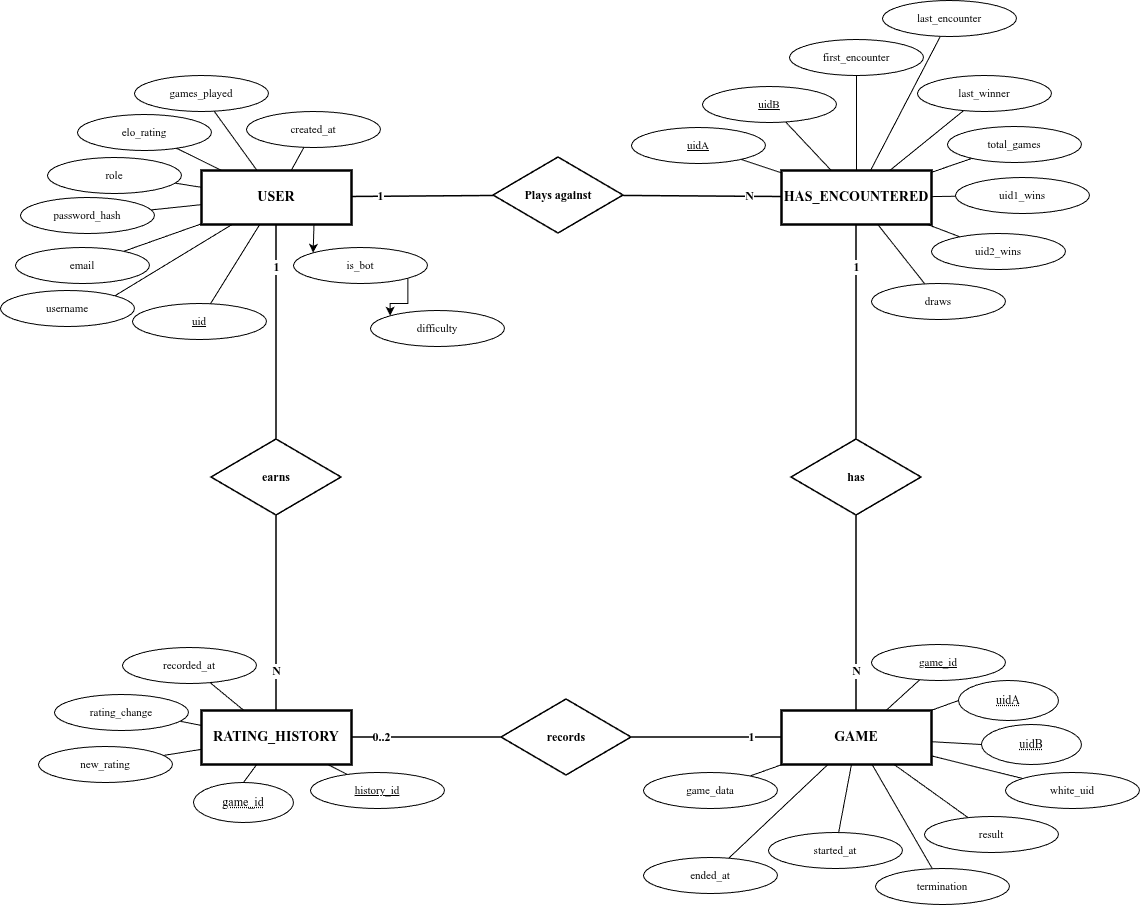
\includegraphics[height=15cm,width=15cm]{client-erd.png}
  \caption{Entity Relationship Diagram of Multiplayer Chess Game}
  \label{fig:client-erd}
\end{figure}

The above figure describes the database of client devices. This ERD has extra attributes for User and less attribute for Rating\_History. User entity need is\_bots to distinguish between bot and another to describe difficulty if they are a bot. Rating\_History does not need uid as it is going to be same for logged in user.


\chapter{GANTT CHART}

\begin{figure}[H]
  \centering
  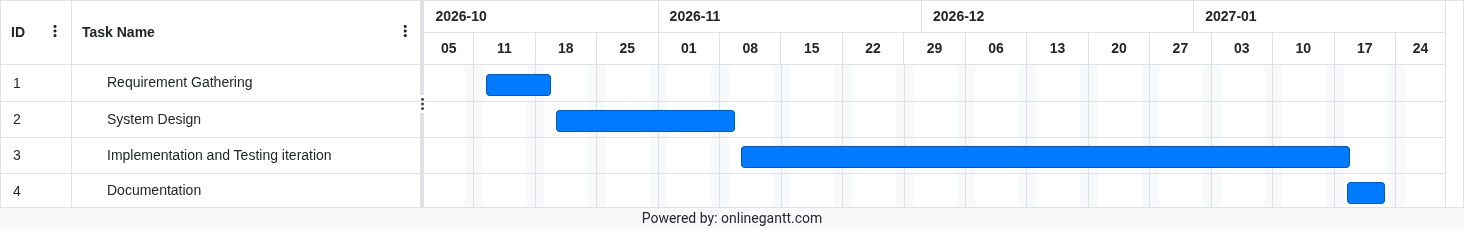
\includegraphics[height=7cm, keepaspectratio,angle=90,scale=0.5]{gantt-chart.png}
  \caption{Gantt Chart of Multiplayer Chess Game}
  \label{fig:gantt}
\end{figure}


\newpage

\chapter{EXPECTED OUTCOMES}
\label{ch:outcomes}

\begin{itemize}[itemsep=2pt]
  \item A fully playable multiplayer chess game with a Raylib-based graphical interface that enforces all standard rules of chess.

  \item A game server that validates moves, synchronizes the game state between players, and prevents illegal moves from being played.

  \item An Elo-based rating and matchmaking system that updates player ratings after every game between players and pairs players of similar skill.

  \item A neural network trained on Lichess games and integrated into the game as a computer AI opponent and offers multiple selectable difficulty levels.

  \item A PostgreSQL database that stores player accounts, games, moves, and rating history, along with game history and leaderboard views for players.

  \item An administrative panel that enables management of players and game records.
\end{itemize}

\textbf{Expected UI}
\begin{figure}[H]
  \centering
  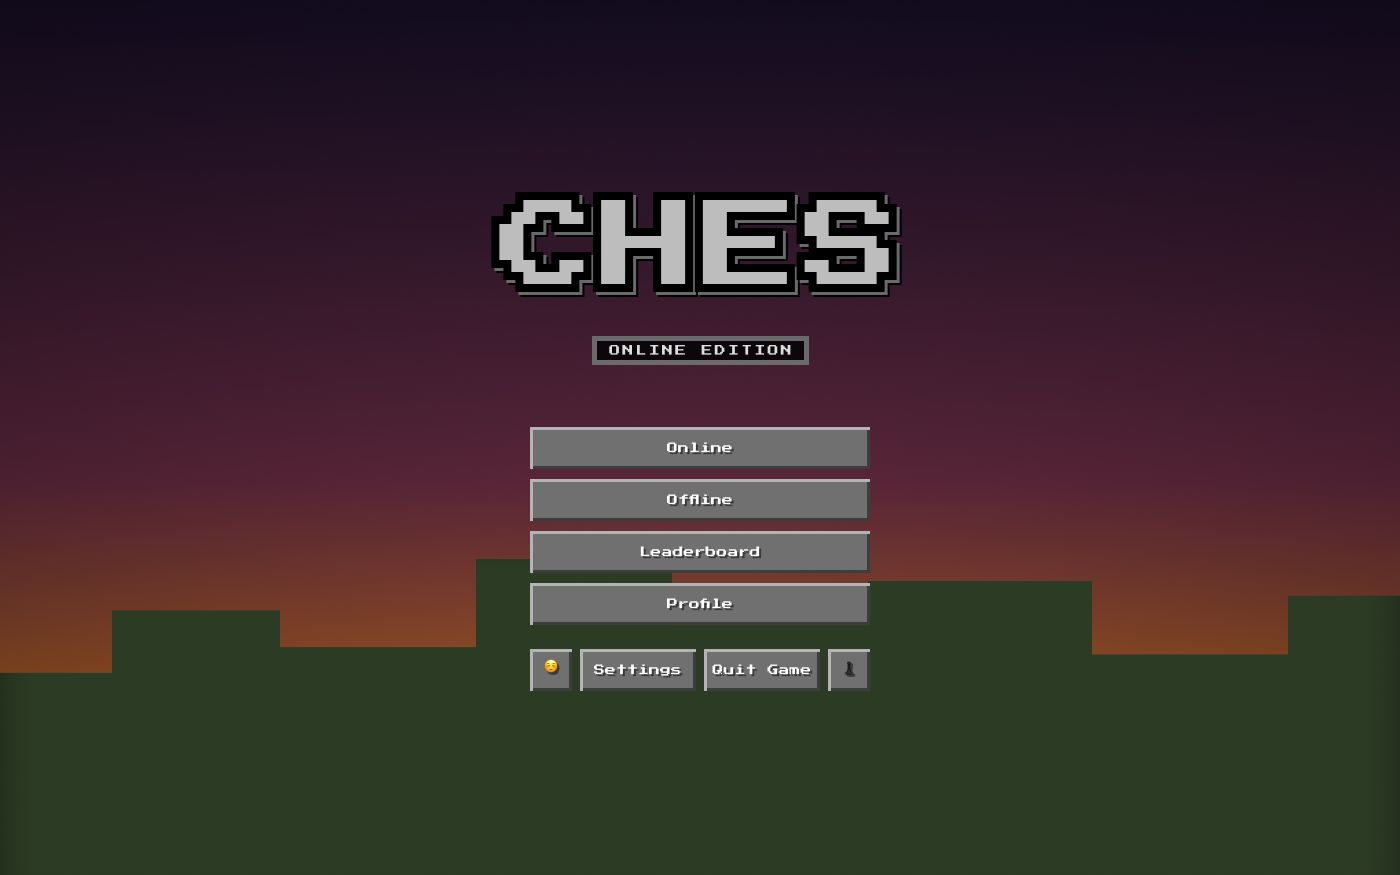
\includegraphics[width=15cm,keepaspectratio]{expected-outcome.jpg}
  \caption{Expected UI of Ches}
  \label{fig:ui}
\end{figure}


\newpage

\chapter{REFERENCES AND BIBLIOGRAPHY}
\label{ch:references}

\bibliographystyle{IEEEtran}

\begingroup
\renewcommand{\chapter}[1]{}
\bibliography{references}
\endgroup

\end{document}
